\documentclass[a4paper,11pt]{article}

\usepackage{../../zyancamlec}
\usepackage{pgfplots}
\usepackage{framed}

\def\ntripos{Mathematical Tripos}
\def\npart{III}
\def\ncourse{Applications of Analysis\\in Physics}
\def\nscourse{AAP}
\def\nlecturer{C.~Warnick}
\def\nterm{Lent}
\def\nyear{2021}

\begin{document}
	\maketitlepage
	\preliminaries

	\section*{Course Information}
	
	This course is aimed at students who are studying physics and are interested in learning some of the more advanced analysis that underpins much of modern theoretical physics. We will emphasise widely applicable concepts and avoid technical details of proofs, while signposting where students can find them. We will aim to cover:

	\begin{itemize}
		\item Background: Hilbert and Banach spaces; distributions; Fourier transform and Sobolev spaces.
	
		\item Compactness: spectra of self-adjoint compact operators; the direct method of the calculus of variations.
	
		\item PDEs on manifolds: Laplace/wave equation on a Riemannian/Lorentzian manifold.
	
		\item Topology and PDEs: index theorems, heat trace.
	\end{itemize}

	\section*{Pre-requisites}

	We assume some basic background analysis knowledge: roughly second year undergraduate level. We also assume some differential geometry at a level similar to that of the GR course.

	\newpage

	\tableofcontents
	\newpage
	\maintext

	\section{Spaces of Functions}

	Many physical quantities are modelled as functions from one space to another.

	\begin{ex}
		\ 
		\begin{itemize}
			\item $\vb x : \mathbb{R} \to \mathbb{R}^3$, i.e.\ $\vb x = \vb x(t)$ describing the trajectory of a particle in 3D;
			\item $\psi : \mathbb{R}^3 \times \mathbb{R} \to \mathbb{C}$, i.e.\ $\psi = \psi(\vb x, t)$ wavefunction;
			\item $(\vb E, \vb B) : \mathbb{R}^3 \times \mathbb{R} \to \mathbb{R}^3 \times \mathbb{R}^3$, E-M field.
		\end{itemize}
	\end{ex}

	Even when a problem requires us to find a single function as its solution, it's often useful to think about a space of possible solutions with a notion of 	`closeness':

	\begin{ex}
		\ 
		\begin{itemize}
			\item Sequences of approximations;
			\item Imperfect measurements mean we can never know data with complete accuracy.
		\end{itemize}
	\end{ex}

	We want to introduce the idea of \emph{topology} to spaces of functions.

	In $\mathbb{R}^n$, we have a standard definition of `nearby', i.e.\ $x$ is near $y$ if 
	\[
		\abs{x-y} = \sqrt{(x_1-y_1)^2 + \cdots + (x_n - y_n)^2}
	\]
	is small. Below, we would say $y$ is \emph{closer} to $x$ than $z$.

	\begin{center}
		\begin{tikzpicture}
			\filldraw[black] (0,0) circle (1pt) node[anchor=west]{$x$};
			\draw[red, dashed] (0,0) circle (30pt);
			\filldraw[black] (0.45,0.5) circle (1pt) node[anchor=west]{$y$};
			\filldraw[black] (3,0) circle (1pt) node[anchor=west]{$z$};
		\end{tikzpicture}
	\end{center}

	For functions we can have many notions of closeness.

	\begin{ex}
		Consider a particle in 1D, acted on by a force $F(t)$ which vanishes for $t<0, t>1$. If particle starts from rest, consider the final momentum
		\[
			\dot{P} = F \quad \Rightarrow \quad P = \int_{0}^{1} F(t) \dd{t}.
		\]
		
		If we repeat experiment for two forces, $F_1, F_2$, then
		\[
			\abs{P_1 - P_2} = \abs{\int_{0}^{1} [F_1 (t) - F_2(t)] \dd{t}} \leq \int_{0}^{1} \abs{F_1 - F_2} \dd{t} =: \norm{F_1 - F_2} _{L^1}.
		\] 
		
		If $\norm{F_1 - F_2}_{L^1}$ is small, then $F_1$ and $F_2$ are `close' in the sense that they produce similar effects on the particle.
	\end{ex}

	\begin{ex}
		$\psi : \mathbb{R}^3 \times \mathbb{R} \to \mathbb{C}$ satisfying 
		\[
			\int _{\mathbb{R}^3} \abs{\psi(x, t)}^2 \dd{x} = 1
		\]
		is a wavefunction for a particle.

		Suppose two distinguishable particles are described by $\psi_1, \psi_2$. Consider $U \subset \mathbb{R}^3$. Let 
		\begin{align*}
			P_i & = \Pr(\text{Particle $i$ is in $U$ at $t= 0$})\\
			& = \int _{U} \abs{\psi(x, 0)}^2 \dd{x}.
		\end{align*}

		Then
		\begin{align*}
			\abs{P_1 - P_2} & = \abs{\int _{U} \left( \abs{\psi_1}^2 - \abs{\psi_2}^2 \right) \dd{x}} \\
			& = \abs{\Re \int _U (\bar \psi_1 - \bar \psi_2) (\psi_1 + \psi_2) \dd{x}}\\
			& \leq \left( \int_U \abs{\psi_1 - \psi_2}^2 \dd{x} \right)^{1/2} \left( \int_U \abs{\psi_1 + \psi_2}^2 \dd{x} \right)^{1/2}
		\end{align*}
		using Cauchy-Schwarz inequality
		\[
			\abs{\int fg \dd{x}} \leq \sqrt{\int \abs{f}^2 \dd{x}} \sqrt{\int \abs{g}^2 \dd{x}}.
		\]
		
		Let 
		\[
			\norm{\psi}_{L^2} = \left( \int_{\mathbb{R}^3} \abs{\psi}^2 \dd{x} \right)^{1/2}
		\]
		then
		\[
			\abs{P_1 - P_2} \leq \norm{\psi_1 - \psi_2}_{L^2} \cdot \norm{\psi_1 + \psi_2}_{L^2}.
		\]
		
		But 
		\[
			\norm{\psi_1 + \psi_2}_{L^2} \leq \norm{\psi_1}_{L^2} + \norm{\psi_2}_{L^2} = 2,
		\]
		hence
		\[
			\abs{P_1 - P_2} \leq 2 \norm{\psi_1 - \psi_2}_{L^2}.
		\]
		
	\end{ex}

	\begin{ex}
		Return to the particle acted on by a force, and suppose $$F(t) = \eta(t) \sin kt$$where $\eta$ is smooth and $\eta(0) = \eta(1) = 0$.

		\begin{center}
			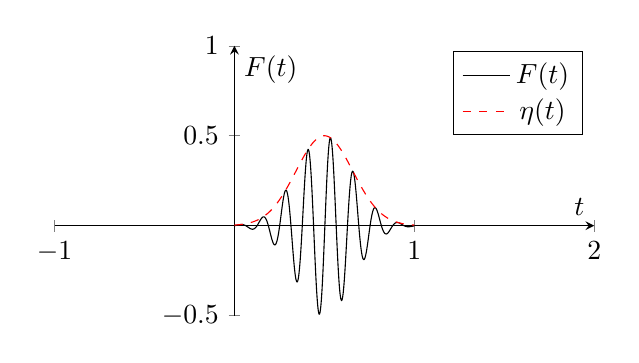
\begin{tikzpicture}
				\begin{axis}[
					axis lines = middle,
					axis equal image,
					xlabel = $t$,
					ylabel = {$F(t)$},
					xmin=-1, xmax=2,
					ymin=-0.5, ymax=1,
					xtick={-1,1,2},
				]
				\addplot [
					domain=0:1, 
					samples=500, 
				]
				{0.5*exp(-20*(x-0.5)^2)*sin(50*deg(x))};
				\addlegendentry{$F(t)$}.
				\addplot [
					domain=0:1, 
					samples=100,
					color=red,
					dashed, 
				]
				{0.5*exp(-20*(x-0.5)^2)};
				\addlegendentry{$\eta(t)$}.
				\end{axis}
			\end{tikzpicture}
		\end{center}

		Then the final momentum is 
		\[
			P = \int_{0}^{1} \eta(t) \sin kt \dd{t} = \int_{0}^{1} \dot{\eta}(t) \frac{\cos kt}{k} \dd{t}
		\]
		so
		\[
			\abs{P} \leq \frac{1}{k} \int_{0}^{1} \abs{\dot{\eta}(t)}\abs{\cos kt} \dd{t} \leq \frac{1}{k} \int_{0}^{1} \abs{\dot \eta(t)} \dd{t} \to 0 \quad \text{as} \quad k \to \infty.
		\]
		
		So $F$ is `close' to $0$ for large $k$, but 
		\[
			\norm{F}_{L^1} = \int_{0}^{1} \abs{\eta(t)} \abs{\sin kt } \dd{t} \not\to 0 \quad \text{as} \quad k \to \infty.
		\]
	\end{ex}
	
	\begin{defi}
		Let $X$ be a vector space over $\mathbb{F} = \mathbb{R}$ or $\mathbb{C}$ (e.g.\ $\mathbb{R}$ or $\mathbb{C}$-valued functions). A \emph{norm} on $X$ is a map $\norm{\cdot} : X \to [0,\infty)$ such that 
		\begin{itemize}
			\item $\norm{x+y} \leq \norm{x} + \norm{y}, \forall x,y \in X$;
			\item $\norm{\lambda y} = \abs{\lambda} \norm{y},  \forall y \in X, \lambda \in \mathbb{F}$;
			\item $\norm{x} \geq 0,  \forall x \in X$ with $\norm{x} = 0 \Leftrightarrow  x = 0$. 
		\end{itemize} 
	\end{defi}

	A norm gives us a notion of convergence: $(x_n)_{n=1}^{\infty} \subset X$ converges to $x \in X$ if for all $\varepsilon > 0$, there exists $N$ s.t.\ $\norm{x_n - x} \leq \varepsilon$ for all $n \geq N$.
	
	\begin{defi}
		$(X, \norm{\cdot})$ is \emph{complete} if every \emph{Cauchy sequence} converges, i.e.\ $(x_n)_{n = 1}^{\infty} \subset X$ has the property that for all $\varepsilon > 0$, there exists $N$ such that $\norm{x_n - x_m} \leq \varepsilon$ for all $n,m \geq N$, then there exists $x \in X$ such that $x_n \to x$.  
	\end{defi}

	\begin{defi}
		A \emph{Banach space} is a complete, normed space.
	\end{defi}

	\begin{ex}
		Notation: $\alpha$ is a multi-index if $\alpha = (\alpha_1, \cdots, \alpha_n)$ with $\alpha_i \in \left\{ 0,1,2,3,\cdots \right\}$. The order of $\alpha$ is $\abs{\alpha} = \alpha_1 + \alpha_2 + \cdots + \alpha_n$, and if $f : \mathbb{R}^n \to \mathbb{C}$, we define the derivative of $f$ with respect to $\alpha$ as 
		\[
			D^\alpha f(x) = \frac{\partial ^{\abs{\alpha}}}{\partial x_1 ^{\alpha_1} \cdots \partial x_n ^{\alpha_n}} f(x).
		\]
		 
		For an open set $U$, define
		\[
			C^k (\bar U) = \left\{ f: U \to \mathbb{C}, \text{$k$ times differentiable}, \sup_U \abs{D^\alpha f} < \infty, \abs{\alpha} \leq k\right\}.
		\]

		This is a Banach space with norm 
		\[
			\norm{f}_{C^k} = \sup _{\substack{x\in U\\\abs{\alpha}\leq k}} \abs{D^\alpha f(x)}.
		\]
	\end{ex}

	\begin{ex}
		If $U \subset \mathbb{R}^n$, then 
		\[
			L^p (U) = \left\{ f : U \to \mathbb{C}\ \Bigg|\ \left( \int _U \abs{f}^p \dd{x} \right)^{1/p} < \infty \right\}
		\]
		with 
		\[
			\norm{f} _{L^p} := \left(\int _U \abs{f}^p \dd{x}\right) ^{1/p}
		\]
		is Banach.
	\end{ex}

	\begin{nt}
		Subtle point: $f$ and $g$ are identified if $f = g$ almost everywhere, i.e.\ $\abs{\left\{ f\neq g \right\}} = 0$.
	\end{nt}

	\subsection{Hilbert Spaces}

	A special case of a Banach space are the Hilbert spaces. Here $H$ is a vector space over $\mathbb{F} = \mathbb{R}$ or $\mathbb{C}$ equipped with an inner product
	\[
		(\cdot, \cdot) = H \times H \to \mathbb{F}
	\]
	satisfying
	\begin{itemize}
		\item $(f,g) = \overline{(g,f)}$;
		\item $(f,\lambda g_1 + g_2) = \lambda(f,g_1) + (f,g_2)$;
		\item $(f,f) \geq 0$ and $(f,f) = 0 \Leftrightarrow f = 0$. 
	\end{itemize}
	Set $\norm{f} = (f,f)^{1/2}$. Require $(H,\norm{\cdot})$ to be Banach.
	
	\begin{ex}
		For $U \subset \mathbb{R}^n$, 
		\[
			L^2(U) = \left\{ f: U \to \mathbb{C}\ \Bigg|\ \left( \int \abs{f}^2 \dd{x} \right)^{1/2} < 0 \right\}
		\]
		we can define
		\[
			(f,g) = \int_U \bar{f} g \dd{x}.
		\]
		(Space of QM states on $U$ is $L^2(U)/\sim$, where $f \sim g$ if $f = \lambda g$, $\lambda \in \mathbb{C}^* = \mathbb{C} \backslash \{0\}$.)
	\end{ex}

	We often want to restrict to `nicer' subspaces of a Banach/Hilbert space, and recover results through approximation.

	We say $D \subset X$ is dense in a Banach space $X$ if for all $x \in X$ and any $\varepsilon > 0$ there exists a $y \in D$ with $\norm{x - y} < \varepsilon$.

	\begin{center}
		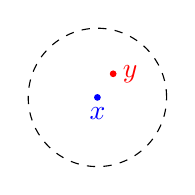
\begin{tikzpicture}
			\filldraw[blue] (0,0) circle (1pt) node[anchor=north]{$x$};
			\draw[dashed] (0,0) circle (25pt);
			\filldraw[red] (0.2,0.3) circle (1pt) node[anchor=west]{$y$};
		\end{tikzpicture}
	\end{center}

	\begin{ex}
		$U \subset \mathbb{R}^n$ us a nice (open) subset of $\mathbb{R}^n$, then 
		\[
			C ^{\infty}_c (U) = \text{``the set of smooth functions vanishing near $\partial U$''}
		\]
		is dense in $L^p(U)$ for $1 \leq p < \infty$.
	\end{ex}

	We can often exploit nice dense subsets to prove results. For example, last lecture we showed that if $\eta$ is smooth and $\eta(0) = \eta(1) = 0$ then
	\[
		\int_{0}^{1} \eta(t) \sin kt \dd{t} \to 0 \quad \text{as} \quad k \to \infty.
	\]

	Suppose instead $\eta \in L^1(0,1)$, i.e.\ $\int_{0}^{1} \abs{\eta} \dd{t} < \infty$. Pick $\tilde \eta \in C ^{\infty}_c ((0,1))$ Then 
	\[
		\int_{0}^{1} \eta(t) \sin kt \dd{t} = \underbrace{\int_{0}^{1} \left( \eta(t) - \tilde \eta(t) \right) \sin kt \dd{t}}_{\leq \varepsilon/2 \text{ by choosing }\tilde \eta} + \underbrace{\int_{0}^{1} \tilde \eta(t) \sin kt \dd{t}}_{\leq \varepsilon/2 \text{ for $k$ large}}
	\]
	by
	\[
		\abs{\int_{0}^{1} \left( \eta(t) - \tilde \eta(t) \right) \sin kt \dd{t}} \leq \norm{\eta - \tilde \eta}_{L^1}.
	\]

	If $X$ has a \emph{countable} dense subset, we say it is \emph{separable}.

	A separable Hilbert space has a countable orthonormal basis, i.e.\ we can find $e_1,e_2, \cdots$ such that 
	\[
		(e_i , e_j) = \delta _{ij}
	\]
	and if $u \in H$ then 
	\[
		u = \sum_i (e_i , u) e_i
	\]
	with the sum converging in the Banach sense.

	Most examples so far are separable.
	
	\subsection{Operators on Banach Spaces}

	Many problems in Physics involve the study of linear operators. If $X$ and $Y$ are Banach spaces, then a linear map $T : X \to Y$ is \emph{bounded} if there exists $C > 0$ such that 
	\[
		\norm{T x}_Y \leq C \norm{x}_X, \quad \forall x \in X.
	\]
	The `best' such $C$ is the operator norm of $T$: 
	\[
		\norm{T}_{\text{op}} : = \sup _{\substack{x \in X\\\norm{x}=1}} \norm{T x}= \sup _{\substack{x \in X\\x\neq 0}} \frac{\norm{T x }}{\norm{x}}.
	\]

	The space $\mathcal{B}(X,Y)$ of bounded linear operators from $X$ to $Y$, with $\norm{\cdot}_{\text{op}}$ is itself a Banach space. If $X = Y$, write $\mathcal{B}(X,X) = \mathcal{B}(X)$.

	\begin{lem}
		\label{lem:1.1}
		Suppose $X,Y$ are Banach, $D \subset X$ is dense and a linear map $T : D \to Y$ satisfies
		\[
			\norm{T x}_Y \leq C \norm{x}_X \quad \forall x \in D
		\]
		then there exists a unique linear map $\bar T : X \to Y$ such that $\norm{\bar T}_{\text{op}} \leq C$
		and $\bar T = T$ on $D$. 

		$\bar T$ is an \emph{extension} of $T$.
	\end{lem}

	\begin{ex}
		$X = C^0 (0,1)$, $D = C^1(0,1)$ 
		\[
			T: D \to \mathbb{C}, \quad Tf := \int_{0}^{1} f'(x)x \dd{x}
		\]
		then 
		\[
			\abs{Tf} = \abs{\int_{0}^{1} f'(x) x \dd{x}} = \abs{\frac{f(1)}{2} - \int_{0}^{1} f(x) \frac{x^2}{2} \dd{x}} \leq \sup _{(0,1)} \abs{f}
		\]
		so $T$ extends uniquely to a map $T : C^0(0,1) \to \mathbb{C}$.
	\end{ex}

	\begin{proof}[Proof sketch of Lemma \ref{lem:1.1}]
		If $x \in X$, take $x_n \to x$ with $x_n \in D$. The boundedness of $T$ implies $T x_n$ converges in $Y$. Set $\bar T x = \lim _{n \to \infty} T x_n$. Check this is well defined.  
	\end{proof}
	
	\begin{ex}
		$X = Y = L^p(0,1)$ with $1 \leq p < \infty$. Take 
		\[
			T : f(x) \mapsto x f(x).
		\]
		This is bounded since 
		\[
			\left( \int \abs{xf}^p \dd{x} \right)^{1/p} = \left( \int_{0}^{1} \abs{x}^p \abs{f(x)}^p \dd{x} \right)^{1/p} \leq \left( \int_{0}^{1} \abs{f(x)}^p \dd{x} \right)^{1/p}
		\]
		i.e.\ $\norm{T f}_{L^p} \leq \norm{f}_{L^p}$. Hence $T \in \mathcal{B}(X)$ and $\norm{T}_{\text{op}} \leq 1$. 

		By considering $f = \chi _{1- 1/n,1}$, one can show that $\norm{T}_{\text{op}} = 1$.

		If $p=2$ this means that the position operator for wavefunctions constrained to $(0,1)$ is bounded.

		\begin{nt}
			$T : f(x) \mapsto xf(x)$ is \emph{not} bounded on $L^p (\mathbb{R})$.
		\end{nt}
	\end{ex}

	\begin{ex}
		Let 
		\[
			G(x,\xi) = \begin{cases}
				(1-\xi) x & x < \xi,\\
				(1-x) \xi & x > \xi.
			\end{cases}
		\]
		
		We can check that 
		\[
			\int_{0}^{1} \int_{0}^{1} \abs{G(x,\xi)}^2 \dd{x}\dd{\xi} = \frac{1}{90}.
		\]

		For $f \in L^2(0,1)$, let 
		\[
			Af(x) = \int_{0}^{1} G(x,\xi) f(\xi) \dd{\xi}.
		\]
		
		By Cauchy-Schwarz inequality, 
		\begin{align*}
			\norm{Af} _{L^2} & = \left( \int_{0}^{1}\abs{\int_{0}^{1} G(x,\xi) f(\xi) \dd{\xi}}^2 \dd{x} \right)^{1/2}\\
			& \leq \left( \int_{0}^{1} \left( \int_{0}^{1} \abs{G(x,\xi)}^2 \dd{\xi} \right) \left( \int_{0}^{1} \abs{f(\xi)}^2 \dd{\xi} \right) \dd{x} \right)^{1/2}\\
			& = \frac{1}{\sqrt{90}} \norm{f}_{L^2}.
		\end{align*}
		
		Hence, $L^2(0,1) \to L^2(0,1)$ is bounded and $\norm{A}_{\text{op}} \leq 1/\sqrt{90}$.

		\begin{nt}
			If $f \in C^0(\overline{(0,1)})$ then $Af = u$ is the unique solution to 
			\[
				-u'' = f, \quad u(0) = u(1) = 0.
			\]
		\end{nt}

		The above gives the steady temperature in a uniform bar, heated at the rate $f(x)$ with endpoints held at $0$. 
	\end{ex}

	\begin{exer}
		Show that $$\norm{A}_{\text{op}} = \frac{1}{\pi^2}.$$ (Hint: assume $f$ can be written as a Fourier series.)
	\end{exer}

	\subsection{Spectra of Bounded Operators}

	For $X$ a Banach space and $T \in \mathcal{B}(X)$, we can obtain important information about $T$ by considering its spectrum. 

	\begin{defi}
		Suppose $T \in \mathcal{B}(X)$. For $\lambda \in \mathbb{C}$, we say $\lambda$ belongs to the \emph{resolvent set} of $T$, $\lambda \in \rho(T)$, if $T - \lambda I : X \to X$ is bijective and $R _{\lambda}(T) = (T - \lambda I)^{-1} : X \to X$ is bounded. If $\lambda \not \in \rho(T)$, then $\lambda$ is in the spectrum of $T$, $\lambda \in \sigma(T)$. 
	\end{defi}

	A point $\lambda$ may belong to $\sigma(T)$ for different reasons:
	\begin{enumerate}[i)]
		\item If $T - \lambda I$ is not injective, there exists $x \in X$ such that $T x = \lambda x$. We say $\lambda$ is an \emph{eigenvalue} of $T$, $x$ an \emph{eigenvector}, we write $\lambda \in \sigma_p(T)$, where $\sigma_p(T)$ is the \emph{point spectrum}.
		\item If $T - \lambda I$ is injective, and the range $\text{Ran}(T - \lambda I)$ is dense in $X$ but not all of $X$, we say $\lambda$ is in the \emph{continuous spectrum} of $T$, $\sigma_c(T)$.
		\item If $T - \lambda I$ is injective, but the range is not dense in $X$, we say $\lambda$ is in the \emph{residual spectrum} $\sigma_r (T)$.
	\end{enumerate}
	Then we see
	\[
		\sigma(T) = \sigma_p(T) \cup \sigma_c(T) \cup \sigma_r(T).
	\]

	\begin{ex}
		If $X = \mathbb{C}^n$ (finite dimensional) then 
		\[
			\sigma(T) = \sigma_p(T) = \left\{ \lambda_1, \lambda_2,\cdots \lambda_n \right\}
		\]
		for $\lambda_i \in \mathbb{C}$ not necessarily distinct.
	\end{ex}

	\begin{ex}
		Recall the position operator $T \in \mathcal{B}\left(L^p(0,1)\right)$ given by $f(x) \mapsto xf(x)$. If $\lambda \not \in [0,1]$, then
		\[
			(T - \lambda I)^{-1} : g(x) \mapsto (x-\lambda)^{-1} g(x)
		\]
		which is a bounded linear operator $L^p(0,1) \to L^p(0,1)$. Hence 
		\[
			\sigma(T) \subset [0,1].
		\]
		
		If $\lambda \in [0,1]$, then $T - \lambda I$ is injective since 
		\[
			(x- \lambda) f(x) = 0  \quad f(x) = 0 \text{ almost everywhere}
		\]
		and 
		\[
			A = \left\{ f \in L^p(0,1)\ |\ f \text{ vanishes in an open neighbourhood of }\lambda \right\} \subset \text{Ran}(T - \lambda I)
		\]
		then $A$ is dense in $L^p(0,1)$, but (for example) $f(x) = 1$ is not in $\text{Ran}(T - \lambda)$. Then
		\[
			\sigma(T) = \sigma_c(T) = [0,1].
		\]
	\end{ex}

	\begin{ex}
		Recall from last ime the operator $A : L^2(0,1) \to L^2(0,1)$
		\[
			G(x,\xi) = \begin{cases}
				(1-\xi)x & x < \xi,\\
				(1-x)\xi & x \geq \xi.
			\end{cases}
		\]
		\[
			A f (x) = \int_{0}^{1}G(x,\xi) f(\xi) \dd{\xi}.
		\]
		\begin{exer}
			Check that if $f_n(x) = \sin n \pi x$, $n = 1,2,\cdots$, then 
			\[
				A f_n = \frac{1}{(n \pi)^2} f_n.
			\]
		\end{exer}
		So $f_n$ are eigenvectors, and $1/(n \pi)^2 \in \sigma_p(A)$, $n = 1,2,\cdots$. 

		In fact 
		\[
			\sigma =  \underbrace{\left\{ \frac{1}{\pi}, \frac{1}{4 \pi^2}, \cdots \right\}}_{\sigma_p} \cup \underbrace{\left\{ 0 \right\}}_{\sigma_c}.
		\]
	\end{ex}
	
	\subsubsection*{Properties of the Spectrum}
	If $T \in \mathcal{B}(X)$, then $\sigma(T)$ is a closed, non-empty subset of $\{ \abs{z} \leq \norm{T}_{\text{op}}\}$. 

	The \emph{spectral radius} is defined to be 
	\[
		r(T) = \sup _{z \in \sigma(T)} \abs{z}
	\]

	\begin{center}
		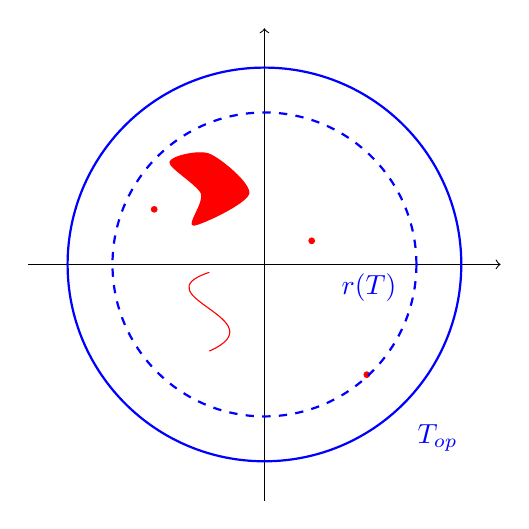
\begin{tikzpicture}
			\draw[->] (-3,0) -- (3,0);
			\draw[->] (0,-3) -- (0,3);
			\filldraw[red] (0.6,0.3) circle (1pt);
			\filldraw[red] (1.3,-1.4) circle (1pt);
			\filldraw[red] (-1.4,0.7) circle (1pt);
			\draw[red] (-0.7,-0.1) .. controls (-1.6,-0.4) and (0.2,-0.7) .. (-0.7,-1.1);
			\filldraw[red] plot[smooth cycle] coordinates{(-0.9,0.5) (-0.8,0.9) (-1.2,1.3) (-0.7, 1.4) (-0.2,0.9)};
			\draw[blue,thick] (0,0) circle (2.5);
			\node[blue] at (2.2,-2.2) {$\norm{T}_{\text{op}}$};
			\draw[blue, thick, dashed] (0,0) circle (1.93);
			\node[blue,anchor=east] at (1.8,-0.3) {$r(T)$};
		\end{tikzpicture}
	\end{center}
	and we have \emph{Gelfand's formula}:
	\[
		r(T) = \lim _{k \to \infty} \norm{T^k}_{\text{op}}^{1/k}.
	\]
	
	\subsection{Self-Adjoint Operators on Hilbert Spaces}

	Suppose $H$ is a Hilbert space with inner product $(\cdot, \cdot)$. A fundamental result: 
	\begin{thm}[Riesz representation theorem]
		If $\Lambda \in \mathcal{B}(H, \mathbb{C})$, then there exists unique $y \in H$ such that 
		\[
			\Lambda x = (y,x), \quad \forall x \in H.
		\]
	\end{thm}

	Now let $T: H \to H$ be a bounded linear operator. For any $y \in H$, the map $\Lambda : x \mapsto (y, Tx)$ is a bounded linear map $\Lambda : H \to \mathbb{C}$ (by Cauchy-Schwarz). So by Riesz representation theorem, there exists $z$ such that $(y, Tx) = (z,x)$ and we write $$z : = T^* y.$$ 
	
	We claim $T^* : H \to H$ is bounded and linear: 
	\begin{align*}
		(y_1 + \lambda y_2 , Tx) & = (y_1, Tx) + \bar \lambda (y_2 , Tx) \\
		& = (T^* y_1 ,x) + \bar \lambda (T^* y_2, x)\\
		& = (T^* y_1 + \lambda T^* y_2, x)\\
		& = (T^* (y_1 + \lambda y_2), x)
	\end{align*}
	so $T^*$ is linear. Also, since (check this)
	\[
		\norm{y} = \sup _{\norm{x} \leq 1} \abs{(x,y)}
	\]
	we see 
	\[
		\norm{T^* y} = \sup _{\norm{x} \leq 1} \abs{(T^* y , x)} = \sup _{\norm{x} \leq 1} \abs{(y , Tx)} \leq \norm{y} \sup _{\norm{x} \leq 1} \norm{T x} = \norm{T}_{\text{op}} \norm{y},
	\]
	therefore, $T^*$ is bounded, $\norm{T^*}_{\text{op}} \leq \norm{T}_{\text{op}}$. We can check that $(T^*)^* = T$ so, in fact $\norm{T}_{\text{op}} = \norm{T^*}_{\text{op}}$.

	We call $T^*$ the \emph{adjoint} of $T$ and if $A \in \mathcal{B}(H)$ with $A^* = A$, then we say $A$ is \emph{self-adjoint} or \emph{Hermitian}.

	\begin{thm}
		If $A \in \mathcal{B}(H)$ is self-adjoint, then $\sigma_r(A) = \0$, $\sigma(A) \subset \mathbb{R}$ and $r(A) = \norm{A}_{\mathrm{op}}$. 
	\end{thm}

	We will move onto the spectral theorem for bounded self-adjoint operators, but first we will consider the \emph{continuous functional calculus}.

	Suppose $T \in \mathcal{B}(H)$. A natural question is when we can define $f(T)$ for some function $f$. 
	
	If $f$ is a polynomial, this is straightforward:
	\[
		f(t) = a_0 + a_1 t + \cdots + a_n t^n, \quad a_i \in \mathbb{C},
	\]
	so we can set 
	\[
		f(T) = a_0 + a_1 T + \cdots + a_n T^n.
	\]

	If $f$ is analytic at $0$, with radius of convergence $R$, we can write 
	\[
		f(t) = \sum _{ n = 0}^{\infty} a_n t^n, \quad \abs{t} < R.
	\]
	
	Now since 
	\[
		\norm{\sum _{n = N}^M a_n T^n}_{\mathrm{op}} \leq \sum _{n = N}^M \abs{a_n} \norm{T}_{\mathrm{op}}^n,
	\]
	if $\norm{T}_{\mathrm{op}} < R$ then 
	\[
		s^N = \sum _{n = 1}^N a_n T^n
	\]
	is a Cauchy sequence in $\mathcal{B}(H)$.

	We can define 
	\[
		f(T) = \sum _{n = 0}^{\infty} a_n T^n
	\]
	for $\norm{T}_{\mathrm{op}} < R$, giving a definition of (for example) $\exp(T), \sin(T)$, etc.
	
	For more general functions, this won't work.
	
	\paragraph{Idea} If $A$ is an $n\times n$ Hermitian matrix, let $e_1, e_2, \cdots, e_n$ be eigenvectors with eigenvalues $\lambda_1, \lambda_2, \cdots \lambda_n$, we can define 
	\[
		f(A) e_i = f(\lambda_i) e_i.
	\]
	which defines $f(A) : \mathbb{C}^n \to \mathbb{C}^n$, works for any function $f$ defined on $\sigma(A)$.

	C.f.\ In the context of Quantum Mechanics, given $A$ an observable, we can write 
	\[
		1 = \sum_i \dyad{\psi_i}{\psi_i}, \quad A \ket{\psi_i} = \lambda_i \ket{\psi_i}.
	\]
	We would like to justify this.

	\subsection{The Continuous Functional Calculus}

	$A : H \to H$ is bounded, self-adjoint operator on a Hilbert space $H$.

	Let $P(t)$ be a polynomial with complex coefficients. We know that $P(A)$ can be defined. We claim $\sigma(P(A)) = P(\sigma(A))$, i.e.\ $\mu$ is in spectrum of $P(A)$ iff $\mu = P(\lambda)$ for $\lambda$ in the spectrum of $A$. To see this, suppose $\lambda \in \sigma(A)$. Then since 
	\[
		P(t) - P(\lambda) = (t - \lambda) Q(t)
	\]
	with $Q$ a polynomial, hence 
	\[
		P(A) - P(\lambda) = (A - \lambda) Q(A)
	\]
	$A - \lambda$ has no bounded inverse, so $P(A) - P(\lambda)$ has no bounded inverse either. Therefore, $P(\lambda) \in \sigma(P(A))$.
	
	Conversely, suppose $\mu \in \sigma(P(A))$. Then 
	\[
		P(t) - \mu = a(t - \lambda_1) \cdots (t - \lambda_n)
	\]
	with $\lambda_1, \cdots, \lambda_n$ roots of $P(t) - \mu$. If $(A - \lambda_i)$ is invertible for $i = 1,\cdots, n$ then $P(A) - \mu$ invertible. So, if $\mu \in \sigma(P(A))$ at least one of $(A - \lambda_1), \cdots, (A - \lambda_n)$ must not be invertible, so there exists $\lambda \in \sigma(A)$ such that $P(\lambda) = \mu$.

	Recall that for a self-adjoint operator $\norm{A}_{\mathrm{op}} = \sup _{\lambda \in \sigma(A)} \abs{\lambda}$. 

	It follows from this, and the calculation above that
	\[
		\norm{P(A)}_{\mathrm{op}} = \sup _{\lambda \in \sigma(A)} \abs{P(\lambda)}.
	\]
	
	We have shown that we have a map $\phi$ from the set of polynomials, with norm $\sup _{\lambda \in \sigma(A)} \abs{P(\lambda)}$ to the set of bounded linear operators on $H$ such that 
	\begin{enumerate}[i)]
		\item If $f(x) = x$, then $\phi(f) = A$;
		\item $\phi(fg) = \phi(f) \phi(g)$, $\phi(\lambda f) = \lambda \phi(f)$, $\phi(1) = I$, $\phi(\bar f) = \phi(f)^*$, i.e.\ $\phi$ is an \emph{algebraic $*$-homomorphism};
		\item $\norm{\phi(f)}_{\mathrm{op}} = \sup _{\lambda \in \sigma(A)} \abs{f(\lambda)}$;
		\item If $f \geq 0$ on $\sigma(A)$, then $\phi(f) \geq 0$ (operator $A$ is positive if $(\psi, A \psi) \geq 0$, $\forall \psi \in H$).  
	\end{enumerate}

	The set of polynomials is dense in $C(\sigma(A))$ --- the space of continuous functions defined on $\sigma(A)$. By a previous lemma, $\phi$ extends uniquely to a map 
	\[
		\phi : C(\sigma(A)) \to \mathcal{B}(H)
	\]
	with the same properties as above.

	\begin{ex}
		If $H = \mathbb{C}^n$ then $A$ has eigenvalues $\lambda_1, \cdots \lambda_n$ (possibly repeated), $C(\sigma(A))$ are simply vectors 
		\[
			\mqty(f_1\\\vdots\\f_n)
		\]
		where $f(\lambda_i) = f_i$.

		Given any such $f$, we can find $P$, a polynomial, with $P(\lambda_i) = f_i$. Then $f(A) = P(A)$. 
	\end{ex}

	\subsection{Spectral Measures}

	Let pick $\psi \in H$, and consider, for $f \in C(\sigma(A))$ the number $(\psi, f(A) \psi)$. 
	
	The map $f \mapsto (\psi, f(A)\psi)$ is linear as $$f + \lambda g \mapsto (\psi, (f + \lambda g)(A) \psi) = (\psi, f(A) \psi) + \lambda (\psi, g(A)\psi).$$
	It is also bounded, 
	\[
		\abs{(\psi, f(A) \psi)} \leq \norm{\psi}^2 \norm{f(A)}_{\mathrm{op}} \leq \norm{\psi}^2 \sup _{\lambda \in \sigma(A)} \abs{f(\lambda)}.
	\]
	It is positive: if $f \geq 0$, then $(\psi, f(A)\psi) \geq 0$.

	We can invoke the \emph{Riesz-Markov theorem}. This tells us that 
	\[
		(\psi, f(A) \psi) = \int _{\sigma(A)} f \dd{\mu_\psi}
	\]
	where $\mu_\psi$ is a \emph{measure}, called the \emph{spectral measure}.

	\begin{framed}
		\textbf{Measures} \ A \emph{measure} assigns a notion of size to subsets of a space. 
		\begin{ex}
			\ 
			\begin{enumerate}[a)]
				\item If $V \subset \mathbb{R}^n$, the volume of $V$ is a measure;
				\item If $\lambda_1, \cdots, \lambda_n \in \mathbb{R}$, then for a set $A \subset \mathbb{R}$, we can define the measure to be the number of $\lambda_i$'s in $A$.
			\end{enumerate}
		\end{ex}

		Corresponding to a measure, we get a notion of \emph{integration}. For the examples above, 
		\begin{enumerate}[a)]
			\item \[
				\int _{\mathbb{R}^n} f(x) \dd{x};
			\]
			\item \[
				\sum _{i = 1}^{n} f(\lambda_i)
			\]
		\end{enumerate}
	\end{framed}

	We can now extend our functional calculus to any integrable function. If we know $(\psi, f(A) \psi)$ for any $\psi$, we can deduce $(\phi, f(A)\psi)$ for any $\phi, \psi$ by \emph{polarisation identity}. 

	C.f.\ if $\vb x, \vb y \in \mathbb{R}^n$, we can write 
	\[
		\vb x \vdot \vb y = \frac{1}{4} \left( \abs{\vb x + \vb y}^2 - \abs{\vb x - \vb y}^2 \right).
	\]
	
	Given $f$ integrable, we define 
	\[
		(\psi, f(A) \psi) = \int _{\sigma(A)} f \dd{\mu_\psi}
	\]
	deduce
	\[
		(\phi, f(A) \psi) = (\phi, \tilde \psi) \quad \text{for} \quad \tilde \psi \in H
	\]
	by Riesz representation. Therefore, $f(A) \psi = \tilde \psi$ is defined.

	Now let us assume there exists a \emph{cyclic vector} $\psi \in H$, i.e.\ a vector such that $\Span\left\{ A^n \psi \right\}$ is dense in $H$. Then we can identify $H$ with $L^2 (\sigma(A), \dd{\mu_\psi})$ such that $A$ acts as the multiplication operator
	\[
		f(\lambda) \mapsto \lambda f(\lambda).
	\]
	 
	To see this, note that the map
	\[
		U: L^2(\sigma(A), \dd{\mu_\psi}) \to H, \quad f \mapsto f(A) \psi
	\]
	is unitary, since 
	\[
		(f(A)\psi, f(A)\psi) = (\psi, \bar f(A) f(A) \psi) = \int _{\sigma(A)} \bar f f \dd{\mu_\psi} = \norm{f}^2 _{L^2 (\sigma(A), \dd{\mu_\psi})}.
	\]
	 
	$U$ is injective, bounded, $\Im(U)$ contains $\Span \{A^n \psi\}$, so $\Im(U)$ is dense, $U^{-1}: \Im(U) \to H$ exists and is bounded. Thus extends to a bounded inverse on $H$ such that $U^{-1}$ is also unitary.

	Therefore, we have a unitary operator which identifies $L^2 (\sigma(A), \dd{\mu_\psi})$ and $H$.

	In general, we may not have a cyclic vector. In this case, we split $H = H_1 \oplus \cdots \oplus H_N$ ($N$ may be $\infty$) such that $A : H_i \to H_i$ and each $H_i$ has a cyclic vector.

	C.f.\ in Quantum Mechanics, for 
	\[
		1 = \sum_i \dyad{\psi_i}{\psi_i}, \quad A \ket{\psi_i} = \lambda_i \ket{\psi_i}
	\]
	we identify
	\[
		\braket{\phi}{\psi} = \underbrace{\sum_i}_{\int \dd{\mu_\psi}} \underbrace{\braket{\phi}{\psi_i}}_{(U^{-1} \phi)^*} \underbrace{\braket{\psi_i}{\psi}}_{U^{-1} \psi}.
	\]
	
	\begin{ex}
		Let 
		\[
			G(x,\xi) = \begin{cases}
				(1 - \xi) x & x < \xi,\\
				(1 - x) \xi & x > \xi.
			\end{cases}
		\]

		For $f \in L^2(0,1)$, define $Af = \int_{0}^{1} G(x, \xi) f(\xi) \dd{\xi}$. Note that $G(x,\xi) = \overline{G(\xi,x)}$. Then
		\begin{align*}
			(g, Af)_{L^2} & = \int_{0}^{1} \bar g(x) \int_{0}^{1} G(x,\xi) f(\xi) \dd{\xi} \dd{x}\\
			& = \int_{0}^{1}\ \overline{\int_{0}^{1} G(\xi, x) g(x) \dd{x}}\ f(\xi) \dd{\xi}\\
			& = (Ag, f) _{L^2}.
		\end{align*}
		Therefore, $A : L^2(0,1) \to L^2(0,1)$ is bounded and self-adjoint. 
	\end{ex}

	Let $H = L^2(0,1)$. Use bra-ket notation: If $\psi \in L^2(0,1)$ then the ket is defined by $\ket{\psi} := \psi$. The bra is defined as 
	\[
		\bra{\psi} = \left( \phi \mapsto (\psi,\phi)_{L^2} \right) \in H^*,
	\]
	and the braket is 
	\[
		\braket{\psi}{\phi} = (\psi, \phi)_{L^2}.
	\]

	Let $\ket{n} = \frac{1}{\sqrt{2}} \sin n\pi x$. Then we have 
	\[
		A \ket{n} = \frac{1}{(n \pi)^2} \ket{n}
	\]
	and $\braket{m}{n} = \delta _{mn}$. Assume $\overline{\Span \{\ket{n}\}} = L^2(0,1)$. 
	
	Recall the spectrum of $A$ 
	\[
		\sigma(A) = \left\{ \frac{1}{\pi^2}, \frac{1}{4 \pi^2}, \frac{1}{9 \pi^2}, \cdots  \right\} \cup \{0\}.
	\]

	A continuous function $f : \sigma(A) \to \mathbb{C}$ is a sequence $(f_n)_{n=1}^{\infty}$ such that $f_n \to f_\infty$ as $n \to \infty$.

	This corresponds to 
	\[
		f\left( \frac{1}{(n \pi)^2} \right) = f_n, \quad f(0) = f _{\infty}.
	\]

	Given $\varepsilon > 0$, pick a polynomial $P$ such that 
	\[
		\abs{P \left( \frac{1}{(n \pi)^2} \right) - f_n} < \varepsilon, \quad \forall n.
	\]
	We know there exists $f(A) \in \mathcal{B}(H)$ such that $\norm{f(A) - P(A)} < \varepsilon$.
	\begin{align*}
		f(A) \ket{n} & = (f(A) - P(A)) \ket{n} + P(A) \ket{n}\\
		& = \ket{R} + P \left( \frac{1}{(n \pi)^2} \right) \ket{n}\\
		& = f_n \ket{n} + \mathcal{O}(\varepsilon) \ket{n} + \ket{R}
	\end{align*}
	and by 
	\[
		\braket{R}{R} \leq \norm{f(A) - P(A)}^2 \norm{n}
	\]
	we have 
	\[
		f(A) \ket{n} = f_n \ket{n} + \ket*{\tilde R}
	\]
	with $\braket*{\tilde R}{\tilde R} = \mathcal{O}(\varepsilon^2)$. Taking $\varepsilon \to 0$, we have 
	\[
		f(A) \ket{n} = f_n \ket{n}.
	\]

	Given $\ket{\psi} \in H$, write 
	\[
		\ket{\psi} = \sum _{n = 1}^{N} \braket{n}{\psi} \ket{n} + \ket{R_N}
	\]
	with $\norm{R_N}^2 < \varepsilon$ and $\braket{n}{R_N} = 0$ for $n \leq N$, provided $N$ is large enough.
	
	\[
		\mel{\psi}{f(A)}{\psi} = \sum _{n = 1}^{N} \abs{\braket{n}{\psi}}^2 f_n + \mel{R_N}{f(A)}{R_N}
	\]
	we can take $N \to \infty$ and deduce
	\[
		\mel{\psi}{f(A)}{\psi} = \sum _{n = 1}^{\infty} f_n \braket{\psi}{n} \braket{n}{\psi}.
	\]
	
	We want 
	\[
		\int _{\sigma(A)} f \dd{\mu_\psi} = \sum _{n = 1}^{\infty} f_n \braket{\psi}{n} \braket{n}{\psi}.
	\]

	Or, in other words,
	\[
		\dd{\mu_\psi} = \sum _{n = 1}^{\infty} \abs{\braket{\psi}{n}}^2 \delta \left( x - \frac{1}{(n \pi)^2} \right) \dd{x}.
	\]
	
	Moreover, if 
	\[
		\sum _{n = 1}^{\infty} \abs{f_n}^2 \abs{\braket{\psi}{n}}^2 < \infty,
	\]
	then
	\[
		f(A) \ket{\psi} = \sum _{ n = 1}^{\infty} f_n \ket{n} \braket{n}{\psi}
	\]
	converges in $H$.
	
	Want to identify $(f_n)$ with the state 
	\[
		\ket*{\hat f} = \sum _{n = 1}^{\infty} f_n \ket{n} \braket{n}{\psi}.
	\]
	Clearly,
	\[
		\braket*{\hat f}{\hat f} = \sum _{n=1}^{\infty}\abs{f_n}^2 \abs{\braket{n}{\psi}}^2
	\]
	is isometry from 
	\[
		\left\{ (f_n)\ \Bigg|\ \sum _{n=1}^{\infty}\abs{f_n}^2 \abs{\braket{n}{\psi}}^2 < \infty\right\} \text{ to $H$}.
	\]

	If $\psi$ is cyclic, then \emph{every} state in $H$ may be written as $\ket*{\hat f}$ for some $(f_n)$. If $\ket{\psi}$ is not cyclic, this is not true. E.g.\ if $\ket{\psi} = \ket{m}$, 
	\[
		\ket*{\hat f} = f_m \ket{m}, \quad \forall (f_n).
	\]

	Or, e.g.\ we can take
	\[
		\ket{\psi} = \sum _{m = 1}^{\infty} 2 ^{- m / 2} \ket{m}
	\]
	which is cyclic.
	
	\subsection{Unbounded Operators}
	Many operators in Quantum Mechanics are not bounded. E.g.\ $\hat x : \psi(x) \mapsto x \psi(x)$ for $\psi \in L^2(\mathbb{R})$, or $\hat p : \psi \mapsto - \mathrm{i} \psi'$. 

	A(n)\ (unbounded) operator on $H$ is a linear map $T$ from its domain, a dense linear subspace of $H$ denoted $D(T)$, to $H$, 
	\[
		T : D(H) \to H, \quad \overline{D(T)} = H, \quad D(T) \leq H.
	\]
	
	\begin{ex}
		\ 
		\begin{enumerate}[a)]
			\item $H = L^2(\mathbb{R})$, take \[
				D(T_1) = \left\{ \varphi \in L^2(\mathbb{R})\ \Bigg|\ \int _{\mathbb{R}} \abs{x}^2 \abs{\varphi}^2 \dd{x} < \infty \right\}
			\]
			and 
			\[
				T_1 : D(T_1) \to H, \quad \varphi(x) \mapsto x \varphi(x).
			\]
			$T_1$ is unbounded since we can make $\norm{T_1 \varphi}$ as large as we like, keeping $\norm{\varphi} = 1$ by translating towards $\infty$.
			\begin{center}
				\begin{tikzpicture}
					\begin{axis}[
						axis lines = middle,
						axis equal image,
						ticks=none,
						ymin=0,ymax=0.4,
					]
					\addplot [
						domain=-0.5:0.5, 
						samples=500, 
						red,
					]
					{0.2*exp(-100*(x)^2)};
					\node[red] at (axis cs:0.25,0.1) {$\norm{\psi} = 1$};
					\end{axis}
				\end{tikzpicture}%
				~%
				%
				\begin{tikzpicture}
					\begin{axis}[
						axis lines = middle,
						axis equal image,
						ticks=none,
						ymin=0,ymax=0.4,
					]
					\addplot [
						domain=0:1, 
						samples=500, 
						blue,
					]
					{0.2*exp(-100*(x-0.7)^2)};
					\node[blue] at (axis cs:0.3,0.1) {$\norm{T_1 \psi} \gg 1$, $\norm{\psi} = 1$};
					\end{axis}
				\end{tikzpicture}
			\end{center}
			\item $H = L^2(\mathbb{R})$, $D(T_2) = C ^{\infty}_c(\mathbb{R})$ and 
			\[
				T_2 : \varphi \mapsto - \mathrm{i} \varphi'
			\]
			$T_2$ is unbounded: take $\varphi = e ^{\mathrm{i} k x} f (x)$, $k \in \mathbb{R}$, then 
			\[
				\norm{\varphi} = \norm{f}, \quad \norm{T_2 \varphi} \sim \abs{k} \norm{f} \to \infty \text{ as } k \to \infty.
			\]
		\end{enumerate}
	\end{ex}

	The \emph{graph} of $T$ is the set of pairs 
	\[
		\Gamma(T) = \left\{ (\varphi, T \varphi)\ |\ \varphi \in D(T) \right\} \subset H \times H.
	\]
	$\Gamma(T)$ is a linear subspace of $H \times H$, which is a Hilbert space with inner product 
	\[
		\expval{(\varphi_1, \psi_1), (\varphi_2, \psi_2)} = \expval{\varphi_1, \varphi_2} + \expval{\psi_1, \psi_2}.
	\]

	If $\Gamma(T)$ is closed, we say $T$ is a \emph{closed operator}. $T : D(T) \to H$ is closed if for any sequence $x_n \in D(T)$ such that $x_n$ and $T x_n$ converge, we have $x = \lim _{n \to \infty} x_n \in D(T)$ and $T x_n \to T x$.

	\begin{ex}
		$T_1$ above is closed, but $T_2$ is \emph{not} closed.
	\end{ex}

	Suppose $T_1, T$ are operators on Hilbert space $H$. If $\Gamma(T_1) \supset \Gamma(T)$ then we say $T_1$ is an \emph{extension} of $T$ and write $T_1 \supset T$.

	\[
		T_1 \supset T \quad \Leftrightarrow \quad D(T_1) \supset D(T) \quad \text{and} \quad T_1 \varphi = T \varphi, \forall \varphi \in D(T).
	\]
	
	\begin{ex}
		$D(T_3) = C^1_c (\mathbb{R})$, $T_3 : \varphi \mapsto - \mathrm{i} \varphi'$ then $T_3 \supset T_2$ because $C^1_c(\mathbb{R}) \supset C ^{\infty}_c (\mathbb{R})$ and if $\varphi \in C ^{\infty}_{c}(\mathbb{R})$ then $T_3 \varphi = T_2 \varphi$.  
	\end{ex}

	$T$ is \emph{closable} if it has a closed extension. A closable operator has a smallest closed extension, $\bar T$ (\emph{closure} of $T$) defined by $\Gamma(\bar T) = \overline{\Gamma(T)}$. 

	$D(\bar T)$ is the set of $x \in H$ such that we can find $x_n \in D(T)$ with $x_n \to x$ and $T x_n \to y$ for some $y \in H$. Then for such an $x$ we set $Tx := y$.
	
	\begin{ex}
		Take $T_2$ above. 
		\[
			D(\bar T_2) = H^1 (\mathbb{R}) = \left\{ u \in L^2(\mathbb{R})\ |\ u' \in L^2(\mathbb{R}) \right\}
		\]
		where $u'$ is the \emph{distributional derivative}.

		Then $\bar T_2 : u \mapsto - \mathrm{i} u'$ is a closed operator.

		$H^1(\mathbb{R})$ is a \emph{Sobolev space}. $u \in H^1(\mathbb{R})$ if $u\in L^2(\mathbb{R})$ and there exists $v \in L^2(\mathbb{R})$ such that 
		\[
			\int _{\mathbb{R}} u \varphi' \dd{x} = - \int _{\mathbb{R}} v \varphi \dd{x}, \quad \forall \varphi \in C ^{\infty}_c (\mathbb{R}).
		\]

		$H^1(\mathbb{R})$ is a Hilbert space with norm
		\[
			\norm{u}_{H^1}^2 = \int _{\mathbb{R}} (\abs{u}^2 + \abs*{u'}^2) \dd{x}.
		\]
		
		This implies $\bar T_2 \supset T_2$ is closed.
	\end{ex}
	
	Suppose $T$ is a closed operator on $H$. $\lambda$ is in the \emph{resolvent set} if $T - \lambda I : D(T) \to H$ is a bijection with a bounded inverse. If $\lambda \not \in \rho(T)$, then $\lambda \in \sigma(T)$, the \emph{spectrum}, which we can decompose into $\sigma_p(T), \sigma_c (T), \sigma_r(T)$ exactly as for bounded operators.

	\begin{ex}
		Let $D(T) = H^1(\mathbb{R})$, then $T: D(T) \to H = L^2(0,1), \varphi \mapsto - \mathrm{i} \varphi'$ is closed.

		\begin{clm}
			$\sigma(T) = \sigma_c(T) = \mathbb{R}$.
		\end{clm}

		Suppose $\Im(k) > 0$, for $f \in L^2(\mathbb{R})$ let
		\[
			\varphi(x) = \mathrm{i} e ^{\mathrm{i} kx} \int_{-\infty}^{x}e ^{-\mathrm{i} k \xi}f(\xi) \dd{\xi}.
		\]
		
		If $\Im(k) < 0$ 
		\[
			\varphi(x) = -\mathrm{i} e ^{\mathrm{i} kx} \int_{x}^{\infty}e ^{-\mathrm{i} k \xi}f(\xi) \dd{\xi}.
		\]

		We can verify that, $$- \mathrm{i} \varphi' - k \varphi = f.$$

		We wish to show that the map $f \mapsto \varphi$ is bounded from $H = L^2(0,1)$ to itself.

		To see this, let $\eta \in L^2(0,1)$, consider 
		\begin{align*}
			\abs{(\eta, \varphi)} &= \abs{\int_{-\infty}^{\infty} \overline{\eta (x)} \varphi(x) \dd{x}}\\
			& = \abs{\int_{-\infty}^{\infty} \overline{\eta(x)} e ^{\mathrm{i} kx} \int_{-\infty}^{x} e ^{-\mathrm{i} k \xi} f(\xi) \dd{\xi} \dd{x}}.
		\end{align*}
		
		Change variables $u = x - \xi, v = \xi$, we have
		\begin{align*}
			\abs{(\eta, \varphi)} &= \abs{\int_{0}^{\infty}\dd{u}\int_{-\infty}^{\infty} \dd{v} \overline{\eta (u + v)} e ^{\mathrm{i} ku} f(v)}\\
			& \leq \left( \int_{0}^{\infty}\dd{u}\int_{-\infty}^{\infty} \dd{v} \abs{\eta(u+v)}^2 e ^{-\Im(k)u} \right)^{1/2} \left( \int_{0}^{\infty}\dd{u}\int_{-\infty}^{\infty} \dd{v} \abs{f(v)}^2 e ^{-\Im(k)u} \right)^{1/2}\\
			& = \frac{\norm{\eta}\norm{f}}{\abs{\Im(k)}}.
		\end{align*}
		This is also true for $\Im k < 0$ by similar computation. Therefore,
		\[
			\abs{(\eta,\varphi)} \leq \frac{\norm{\eta}\norm{f}}{\abs{\Im(k)}}, \quad \forall \eta \in H.
		\]
		Set $\eta = \varphi$ , then
		\[
			\norm{\varphi} \leq \frac{\norm{f}}{\abs{\Im(k)}}.
		\]
		Therefore, if $\Im(k) \neq 0$, then $(T - kI) : D(T) \to H$ has a bounded inverse. Then, we conclude 
		\[
			\left\{ \Im(k) \neq 0 \right\} \subset \rho(T).
		\]
		
		Suppose $k \in \mathbb{R}$. Let 
		\[
			\varphi(x) = \eta \left( \frac{x}{R} \right) e ^{\mathrm{i} k x}, \quad \eta \in C ^{\infty}_c (\mathbb{R}).
		\]
		Then 
		\[
			- \mathrm{i} \varphi' - k \varphi = \frac{1}{R} \eta' \left( \frac{x}{R} \right) e ^{\mathrm{i} k x}.
		\]
		Thus
		\begin{align*}
			\norm{(T - k I)\varphi}_{L^2}^2 & = \frac{1}{R^2} \int_{-\infty}^{\infty} \left( \eta' \left( \frac{x}{R} \right) \right) ^2 \dd{x}\\
			& = \frac{1}{R} \norm{\eta'}^2 _{L^2}.
		\end{align*}
		However, 
		\begin{align*}
			\norm{\varphi}_{L^2}^2 = \int_{-\infty}^{\infty} \left( \eta \left( \frac{x}{R} \right) \right)^2 \dd{x} = R \norm{\eta}_{L^2}^2
		\end{align*}
		so $T - kI$ cannot have a bounded inverse. If this were the case, $\psi = R ^{1/2} (T - k)\varphi$, we'd have
		\[
			\norm{\psi}_{L^2} = C \quad \text{(independent of $R$)},
		\]
		\[
			\norm{(T - k)^{-1} \psi} _{L^2} = R C' \quad \text{($C'$ independent of $R$)}.
		\]
		 
		If there exists $K$ such that 
		\[
			\norm{(T - k)^{-1} \psi}_{L^2} \leq K \norm{\psi}_{L^2}
		\]
		we can get a contradiction. Thus $T - k$ has no bounded inverse or $k \in \mathbb{R}$.

		It's easy to see that $(T - kI) \varphi = 0$ then $\varphi = e ^{\mathrm{i} kx} \not \in H$, so $k$ is not in the point spectrum for $k \in \mathbb{R}$. If a) $f \in C ^{\infty}_c (\mathbb{R})$ satisfies 
		\[
			\text{b)} \quad \int _{\mathbb{R}} e ^{- \mathrm{i} k \xi}f(\xi) \dd{\xi} = 0,
		\]
		then 
		\[
			\varphi = e ^{\mathrm{i} kx} \int_{-\infty}^{x} e ^{- \mathrm{i} k \xi} f(\xi) \dd{\xi}
		\]
		gives an inverse to $(T - kI)$. Functions satisfying a), b) are dense in $L^2(0,1)$, so $k\in \sigma_c(T)$ for any $k\in \mathbb{R}$.
	\end{ex}

	\subsection{Adjoints and Self-Adjointness}

	Suppose $T : D(T) \to H$ is a densely defined operator. Let $D(T^*)$ be the set of $\varphi \in H$ such that 
	\[
		\abs{(\varphi, T \psi)} \leq C \norm{\varphi}, \quad \forall \psi \in D(T).
	\]
	
	Then the map $\Lambda : D(T) \to \mathbb{C}$ given by $\Lambda(\psi) = (\psi, T \psi)$ is bounded. Since $D(T)$ is dense this extends uniquely to a linear map from $\Lambda : H \to \mathbb{C}$, so by Riesz representation theorem, there exists a unique $\eta \in H$ such that 
	\[
		(\varphi, T \psi) = (\eta, \psi).
	\]
	
	We define $T^* \varphi := \eta$. $T^*$ is the \emph{adjoint} of $T$.

	\begin{nt}
		\ 
		\begin{itemize}
			\item $T^*$ is closed;
			\item $T$ is closable iff $D(T^*)$ is dense in $H$, then $\bar T = T ^{**}$;
			\item If $T$ is closable, then $(\bar T)^* = T^*$.
		\end{itemize}
	\end{nt}

	\begin{ex}
		\[
			D(T) = \left\{ \varphi \in L^2(\mathbb{R}) : \norm{x}\varphi \in L^2(\mathbb{R}) \right\},
		\]
		\[
			T : D(T) \to H = L^2(\mathbb{R}), \quad \psi \mapsto (a + bx) \psi, \qquad a,b \in \mathbb{C}.
		\]
			 
		Let $\varphi \in H$. Then 
		\[
			(\varphi, T \psi) = \int_{- \infty}^{\infty} \bar{\varphi} (x) (a + bx) \psi(x) \dd{x}.
		\]
		
		Claim that if $\varphi \in D(T)$, then $\varphi \in D(T^*)$ since 
		\begin{align*}
			\abs{(\varphi, T \psi)} & \leq \left( \int_{-\infty}^{\infty} \abs{a + bx}^2 \abs{\varphi}^2 \dd{x} \right)^{1/2} \left( \int_{-\infty}^{\infty} \abs{\psi}^2 \dd{x} \right)^{1/2}\\
			& \leq C \norm{\psi}.
		\end{align*}
		$D(T) \subset D(T^*)$. 
		
		Suppose $\varphi \in D(T^*)$, then 
		\[
			\abs{((\bar a + \bar b x)\varphi, \psi)} \leq C \norm{\psi}, \quad \psi \in L^2,
		\]
		implying
		\[
			(\bar a + \bar b x) \varphi \in L^2.
		\]
		
		Since $\varphi \in L^2$, $x \varphi \in L^2$, $(b \neq 0)$. Thus 
		\[
			D(T^*) = D(T) \quad \text{and} \quad T^* : \varphi \mapsto (\bar a + \bar b x) \varphi.
		\]
	\end{ex}

	\subsubsection{Symmetric and Self-Adjoint Operators}

	A densely defined operator is \emph{symmetric} if $T \subset T^*$, i.e.\ $D(T) \subset D(T^*)$ and $T \varphi = T^* \varphi$, for all $\varphi \in D(T)$, equivalently, $T$ symmetric if 
	\[
		(T \varphi, \psi) = (\varphi, T \psi), \quad \forall \varphi, \psi \in D(T).
	\]
	
	$T$ is \emph{self-adjoint} if $T = T^*$, i.e.\ $T$ is symmetric and $D(T) = D(T^*)$.

	\begin{ex}
		Let $D(T_1) = C ^{\infty}_c(\mathbb{R}) \subset L^2(\mathbb{R})$ and 
		\[
			T_1 : D(T_1) \to L^2(\mathbb{R}),\quad \varphi \mapsto -\mathrm{i} \varphi'.
		\]
		$T_1$ is symmetric:
		\[
			\int _{\mathbb{R}} = \bar \psi(-\mathrm{i} \varphi') \dd{x} = \int _{\mathbb{R}} \overline{(-\mathrm{i} \psi')} \varphi \dd{x}, \quad \forall \varphi,\psi \in D(T_1).
		\]
		
		$T_1$ is \emph{not} self-adjoint: $T_1$ is not closed, but $T_1^*$ is closed, so $T_1 \neq T_1^*$ since $D(T_1)\neq D(T_1^*)$.

		If instead we consider $D(T_2) = H^1(\mathbb{R})$, 
		\[
			T_2 : D(T_2) \to L^2(\mathbb{R}), \quad \varphi \mapsto - \mathrm{i} \varphi'.
		\]
		
		Suppose $\psi \in L^2(\mathbb{R})$ satisfies
		\[
			\abs{(\psi, - \mathrm{i} \varphi')} \leq C \norm{\varphi}, \quad \varphi \in H^1(\mathbb{R}),
		\]
		by Riesz, there exists $\tilde \psi \in L^2(\mathbb{R})$ such that
		\[
			(\psi, - \mathrm{i} \varphi') = (\tilde \psi, \varphi), \quad \forall \varphi \in C ^{\infty}_c (\mathbb{R}) \subset H^1(\mathbb{R}).
		\]
		
		This is precisely the condition that $\psi \in H^1(\mathbb{R})$. Thus $D(T_2) = D(T_2^*)$ and $T_2$ is self-adjoint. 
		 
	\end{ex}
	
	  
\end{document} 